\documentclass[aspectratio=169, 10pt]{beamer}

% --- Packages ---
\usepackage[utf8]{inputenc}
\usepackage[T1]{fontenc}
\usepackage{lmodern}
\usepackage{graphicx}
\usepackage{booktabs}
\usepackage{tikz}
\usetikzlibrary{shapes,arrows,positioning,shadows,fit,backgrounds}
\usepackage{amsmath,amssymb}
\usepackage{hyperref}
\usepackage{xcolor}
\usepackage{colortbl}

% Custom symbols for comparison tables
\newcommand{\ok}[1]{{\color{green!60!black}\textbf{\checkmark}\ \scriptsize #1}}
\newcommand{\ko}{{\color{red!70!black}\textbf{$\times$}}}

% --- Custom Theme/Style Definition ---
% Professional & Modern color palette (Deep Navy & Accent Gold/Cyan)
\definecolor{primaryBlue}{HTML}{0A2540}       % Dark professional navy
\definecolor{secondaryBlue}{HTML}{0070F3}     % Vibrant modern blue
\definecolor{accentGold}{HTML}{FFB000}        % Warm highlight gold
\definecolor{textDark}{HTML}{2D3748}          % Clean charcoal text
\definecolor{bgLight}{HTML}{F8FAFC}           % Soft off-white background
\definecolor{cardBg}{HTML}{FFFFFF}            % Pure white for cards/blocks
\definecolor{borderLight}{HTML}{E2E8F0}       % Subtle borders

% Apply global colors
\setbeamercolor{background canvas}{bg=bgLight}
\setbeamercolor{normal text}{fg=textDark}
\setbeamercolor{structure}{fg=primaryBlue}
\setbeamercolor{alerted text}{fg=accentGold}

% Fonts
\usefonttheme{professionalfonts}
\setbeamerfont{title}{size=\LARGE, series=\bfseries}
\setbeamerfont{subtitle}{size=\large, shape=\itshape}
\setbeamerfont{frametitle}{size=\Large, series=\bfseries}
\setbeamerfont{author}{size=\normalsize}
\setbeamerfont{institute}{size=\small}
\setbeamerfont{date}{size=\small}

% Disable navigation symbols
\setbeamertemplate{navigation symbols}{}

% Custom Bullet Points
\setbeamertemplate{itemize items}[circle]
\setbeamercolor{itemize item}{fg=secondaryBlue}
\setbeamercolor{itemize subitem}{fg=primaryBlue}

% Custom Block Styling (Modern Cards)
\setbeamercolor{block title}{bg=primaryBlue, fg=white}
\setbeamercolor{block body}{bg=white, fg=textDark}
\setbeamertemplate{blocks}[rounded][shadow=true]

% Title Page Customization
\setbeamertemplate{title page}{
    \begin{tikzpicture}[remember picture,overlay]
        % Background geometric shapes
        \fill[primaryBlue] (current page.south west) rectangle ([xshift=0.35\paperwidth]current page.north west);
        \path[fill=secondaryBlue, opacity=0.8] (current page.south west) -- ([xshift=0.35\paperwidth]current page.south west) -- ([xshift=0.25\paperwidth]current page.north west) -- cycle;
        
        % Logo placement in top-left
        \node[anchor=north west, xshift=1.2cm, yshift=-0.6cm] at (current page.north west) {
            
\includegraphics[height=1.4cm]{Logo_IIITL.png}
        };
        
        % Title & Subtitle in the main content area (right side)
        \node[anchor=west, text width=0.58\paperwidth, align=left, xshift=0.38\paperwidth, yshift=1.3cm] at (current page.west) {
            \begin{minipage}{\linewidth}
                \flushleft
                % Left accent bar
                \begin{tikzpicture}[baseline=(T.base)]
                    \node(T)[inner sep=0pt, outer sep=0pt, align=left, text width=0.55\paperwidth]{
                        {\color{primaryBlue}\usebeamerfont{title}\inserttitle}\par
                        \ifx\insertsubtitle\@empty\else
                            \vspace{0.25cm}
                            {\color{secondaryBlue!80}\usebeamerfont{subtitle}\insertsubtitle}\par
                        \fi
                    };
                    \draw[secondaryBlue, line width=4pt] ([xshift=-12pt]T.north west) -- ([xshift=-12pt]T.south west);
                \end{tikzpicture}
            \end{minipage}
        };
        
        % Author & Metadata in the main content area (lower right)
        \node[anchor=south west, text width=0.58\paperwidth, align=left, xshift=0.38\paperwidth, yshift=0.9cm] at (current page.south west) {
            {\color{secondaryBlue}\textbf{\usebeamerfont{author}\insertauthor}}\par\vspace{0.15cm}
            {\color{textDark!85}\usebeamerfont{institute}\insertinstitute}\par\vspace{0.35cm}
            {\color{textDark!50}\usebeamerfont{date}\insertdate}
        };
    \end{tikzpicture}
}

% Header (Frametitle) Styling
\setbeamertemplate{frametitle}{
    \nointerlineskip
    \begin{beamercolorbox}[wd=\paperwidth,ht=1.2cm,dp=0.4cm]{}
        \begin{tikzpicture}[remember picture,overlay]
            \fill[primaryBlue] (current page.north west) rectangle ([yshift=-1.2cm]current page.north east);
            \fill[secondaryBlue] (current page.north west) rectangle ([xshift=0.08\paperwidth, yshift=-1.2cm]current page.north west);
            \node[anchor=west, xshift=0.12\paperwidth, yshift=-0.6cm] at (current page.north west) {
                \color{white}\usebeamerfont{frametitle}\insertframetitle
            };
            % Small logo on the right side of headers
            \node[anchor=east, xshift=-0.4cm, yshift=-0.6cm] at (current page.north east) {
                
\includegraphics[height=0.8cm]{Logo_IIITL.png}
            };
        \end{tikzpicture}
    \end{beamercolorbox}
    \vspace{0.3cm}
}

% Footer (Footline) Styling
\setbeamertemplate{footline}{
    \begin{beamercolorbox}[wd=\paperwidth,ht=0.6cm,dp=0.2cm]{}
        \begin{tikzpicture}[remember picture,overlay]
            \fill[primaryBlue!10] (current page.south west) rectangle (current page.south east);
            \draw[secondaryBlue, line width=1.5pt] (current page.south west) -- (current page.south east);
            
            % Left footline: Institution
            \node[anchor=west, xshift=0.5cm, yshift=0.3cm] at (current page.south west) {
                \tiny\color{primaryBlue!80}\insertshortinstitute
            };
            
            % Center footline: Slide Title
            \node[anchor=center, yshift=0.3cm] at (current page.south) {
                \tiny\color{primaryBlue!80}\insertshorttitle
            };
            
            % Right footline: Page Numbers
            \node[anchor=east, xshift=-0.5cm, yshift=0.3cm] at (current page.south east) {
                \tiny\color{primaryBlue!80}\insertframenumber{} / \inserttotalframenumber
            };
        \end{tikzpicture}
    \end{beamercolorbox}
}

% --- Presentation Info ---
\title[Agricultural Expert System]{Toward a Next Generation \\ Agricultural Expert System}
\subtitle{A Multimodal Conversational Approach}
\author[Shajid Ali Khan]{Shajid Ali Khan}
\institute[IIIT Lucknow]{
    \textbf{Supervisor:} Dr. Deepak Kumar Singh \\
    \vspace{0.2cm}
    Department of Computer Science \\
    Indian Institute of Information Technology, Lucknow
}
\date{\today}

% --- Document Content ---
\begin{document}

% Title Frame
\begin{frame}[plain]
    \titlepage
\end{frame}

% Frame 1: Outline
\begin{frame}{Outline}
    \tableofcontents
\end{frame}

% Frame 2: Introduction
\section{Introduction}
\begin{frame}{Introduction: The Agricultural Advisory Crisis in India}
    \begin{itemize}
        \item \textbf{Extension Shortage:} Only 1 extension worker per 1,000+ farmers in India --- 146 million farm households make critical crop decisions with zero professional guidance \cite{icar2023}.
        \item \textbf{Crop Loss:} 26--30\% of annual crop production is lost to disease and pests, yet most farmers identify symptoms by eye --- well past the optimal treatment window \cite{fao2022}.
        \item \textbf{Data Inaction:} 230 million Soil Health Cards issued but only 14.6\% of farmers acted on them --- no system translates soil data into actionable advice in their own language \cite{nabard2023}.
        \item \textbf{Price Gap:} Farmers sell 30--40\% below optimal price due to lack of real-time mandi data and price forecasting --- a gap affecting over 120 million households \cite{enam2023}.
        \item \textbf{Access Barriers:} Existing agricultural AI is English-only, text-only, and connectivity-dependent --- structurally inaccessible to the majority of Indian farmers it claims to serve.
    \end{itemize}
\end{frame}

% Frame 3: Related Work & Research Gaps
\section{Related Work \& Research Gaps}
\begin{frame}{Related Work \& Research Gaps}
    \centering
    \vspace{-0.2cm}
    \renewcommand{\arraystretch}{1.25}
    \resizebox{1.0\textwidth}{!}{
        \begin{tabular}{llcccccccc}
            \toprule
            \textbf{System} & \textbf{Venue} & \shortstack{\textbf{Multi-agent} \\ \textbf{Router}} & \shortstack{\textbf{VLM} \\ \textbf{Disease}} & \shortstack{\textbf{Soil} \\ \textbf{Sensor}} & \shortstack{\textbf{Weather} \\ \textbf{Prediction}} & \shortstack{\textbf{XAI} \\ \textbf{Farmer UI}} & \shortstack{\textbf{Voice /} \\ \textbf{Indic}} & \shortstack{\textbf{Market} \\ \textbf{Price}} & \textbf{Deployed} \\
            \midrule
            Farmer.Chat \cite{farmerchat2024} & ACM 2024 & \ko & \ko\ (Generic) & \ko & \ok{API} & \ko & \ok{Partial} & \ko & \ok{565k users} \\
            AgroAskAI \cite{agroaskai2024} & arXiv 2024 & \ok{Chain} & \ko & \ko & \ok{Dedicated} & \ko & \ok{Partial} & \ko & \ko \\
            AgriGPT \cite{agrigpt2025} & arXiv 2025 & \ok{Data engine} & \ok{VL ext.} & \ko & \ok{Partial} & \ko & \ko & \ko & \ko \\
            AgriM-LLM \cite{agrimllm2026} & Preprints 2026 & \ko & \ok{Best VE} & \ko & \ko & \ko & \ko & \ko & \ko \\
            \rowcolor{secondaryBlue!10} \textbf{AgriDoctor (Base)} \cite{agridoctor2025} & IEEE 2025 & \ok{Router+5} & \ok{Strong} & \ko & \ko & \ko & \ok{CN/EN only} & \ko & \ko \\
            AgriBuddy \cite{agribuddy2025} & BRAC 2025 & \ok{Partial} & \ok{CNN rice} & \ko & \ok{Partial} & \ko & \ko & \ko & \ok{Partial} \\
            PhenoAssistant \cite{phenoassistant2026} & Nature 2026 & \ok{Yes} & \ok{Research} & \ko & \ko & \ko & \ko & \ko & \ko\ (Lab) \\
            Agentic AI \cite{agenticmdpi2026} & MDPI 2026 & \ok{4 agents} & \ok{Rice CNN} & \ok{Partial} & \ok{Dedicated} & \ko & \ko & \ko & \ko \\
            \bottomrule
        \end{tabular}
    }
    \vspace{0.15cm}
    \begin{block}{\footnotesize Key Research Gaps Identified}
        \footnotesize
        \begin{itemize}
            \item \textbf{Soil Sensor Fusion} and \textbf{Market Price} features are completely missing from existing systems.
            \item No prior platform supports explainable AI (\textbf{XAI}) for farmer UIs or comprehensive \textbf{Indic speech} interfaces.
        \end{itemize}
    \end{block}
\end{frame}

% Frame 5: Problem Statement
\section{Problem Statement}
\begin{frame}{Problem Statement}
    \vspace{0.8cm}
    \setbeamercolor{problemBox}{bg=secondaryBlue!10, fg=textDark}
    \begin{beamercolorbox}[wd=\textwidth, rounded=true, shadow=true, sep=0.4cm]{problemBox}
        Current agricultural AI systems are fatally fragmented: deployed chatbots lack visual diagnostics, advanced vision models lack interactive conversational interfaces, multi-agent setups ignore live market data, and none deliver explainable advice in native Indic languages. Consequently, no existing framework integrates speech, image, soil sensors, weather prediction and live market data into a single trustworthy session.
    \end{beamercolorbox}
\end{frame}

% Frame 6: Research Objectives
\section{Research Objectives}
\begin{frame}{Research Objectives}
    \small
    \begin{itemize}
        \setlength{\itemsep}{0.3ex}
        \item \textbf{O1: Multi-Agent Orchestration} --- Design a LangGraph orchestrator to classify farmer query intent and route requests to domain-specific specialist agents.
        \item \textbf{O2: Disease \& Nutrient Diagnostics} --- Fine-tune a ViT-L/16 (LoRA) model for disease identification ($>90\%$ accuracy) and fuse leaf image features with soil sensor telemetry.
        \item \textbf{O3: Grounded RAG \& Explainable AI} --- Build a BM25/dense vector RAG pipeline over 250k+ documents with LLM confidence gating, surfacing Grad-CAM and SHAP explanations.
        \item \textbf{O4: Speech, Weather \& Market Advisory} --- Implement a 10-language Indic Whisper/Bhashini voice pipeline; deploy an LSTM-based 7-day weather forecasting module using IMD data; and integrate live eNAM prices with Prophet-based mandi price forecasts.
        \item \textbf{O5: Agronomic Benchmarking \& Validation} --- Evaluate system performance against MIRAGE \cite{mirage2025}/AgMMU \cite{agmmu2025} benchmarks and validate real farmer queries with 10 ICAR agronomists.
    \end{itemize}
\end{frame}

% Frame 7: System Architecture
\section{System Architecture}
\begin{frame}{System Architecture}
    \vspace*{-0.55cm}
    \centering
    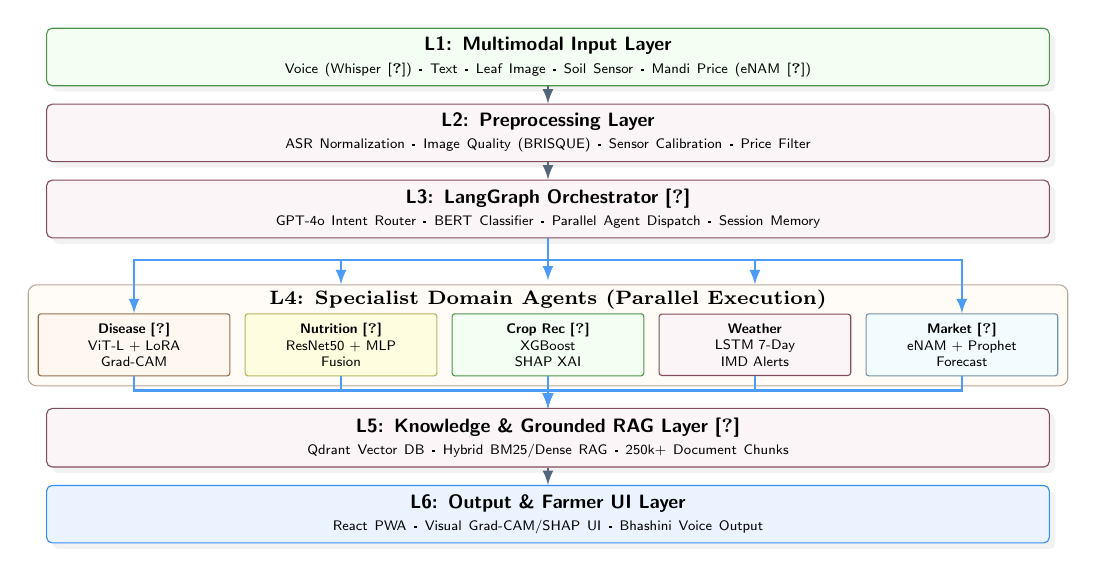
\begin{tikzpicture}[
        node distance=0.22cm and 0.18cm,
        layer/.style={rounded corners=2pt, drop shadow={opacity=0.1}, text width=12.5cm, align=center, font=\scriptsize\sffamily, minimum height=0.5cm},
        agent/.style={rounded corners=1pt, text width=2.2cm, align=center, font=\tiny\sffamily, minimum height=0.7cm}
    ]
        % Layer nodes with exact colors from HTML style
        % L1 Input: lr-t style (soft green)
        \node (l1) [layer, draw=green!40!black!70, fill=green!5!white] {\textbf{L1: Multimodal Input Layer} \\ \tiny Voice (Whisper \cite{indicAsr2025}) · Text · Leaf Image · Soil Sensor · Mandi Price (eNAM \cite{enam2023})};
        
        % L2 Preprocessing: lr-p style (soft purple/lavender)
        \node (l2) [layer, below=of l1, draw=purple!40!black!70, fill=purple!4!white] {\textbf{L2: Preprocessing Layer} \\ \tiny ASR Normalization · Image Quality (BRISQUE) · Sensor Calibration · Price Filter};
        
        % L3 Orchestrator: lr-p style (soft purple/lavender)
        \node (l3) [layer, below=of l2, draw=purple!40!black!70, fill=purple!4!white] {\textbf{L3: LangGraph Orchestrator \cite{agroaskai2024}} \\ \tiny GPT-4o Intent Router · BERT Classifier · Parallel Agent Dispatch · Session Memory};
        
        % Agent Layer (L4)
        \node (a3) [agent, below=0.95cm of l3, draw=green!40!black!70, fill=green!5!white] {\textbf{Crop Rec \cite{xaiCrop2024}}\\ XGBoost \\ SHAP XAI};
        \node (a2) [agent, left=of a3, draw=yellow!60!black!80, fill=yellow!12!white] {\textbf{Nutrition \cite{cropibot2026}}\\ ResNet50 + MLP \\ Fusion};
        \node (a1) [agent, left=of a2, draw=orange!40!black!70, fill=orange!6!white] {\textbf{Disease \cite{llmiCdp2025}}\\ ViT-L + LoRA \\ Grad-CAM};
        \node (a4) [agent, right=of a3, draw=purple!40!black!70, fill=purple!4!white] {\textbf{Weather}\\ LSTM 7-Day \\ IMD Alerts};
        \node (a5) [agent, right=of a4, draw=cyan!40!black!70, fill=cyan!5!white] {\textbf{Market \cite{enam2023}}\\ eNAM + Prophet \\ Forecast};
        
        % Group agents under L4 container box (using backgrounds and fit)
        \begin{scope}[on background layer]
            \coordinate (a3_top) at ([yshift=0.24cm]a3.north);
            \node[draw=orange!30!black!40, fill=orange!3!white, rounded corners=3pt, inner sep=0.12cm, fit=(a1) (a5) (a3_top)] (l4_container) {};
        \end{scope}

        % L4 label node drawn slightly above the container at the top center
        \node[font=\scriptsize\bfseries\color{black}, anchor=north, yshift=0.05cm] (l4_title) at (l4_container.north) {L4: Specialist Domain Agents (Parallel Execution)};
        
        % L5 Knowledge + RAG: lr-p style (soft lavender) - increased gap to 0.40cm
        \node (l5) [layer, below=0.40cm of a3, draw=purple!40!black!70, fill=purple!4!white] {\textbf{L5: Knowledge \& Grounded RAG Layer \cite{ragMaize2026}} \\ \tiny Qdrant Vector DB · Hybrid BM25/Dense RAG · 250k+ Document Chunks};
        
        % L6 Output: lr-b style (soft blue)
        \node (l6) [layer, below=of l5, draw=secondaryBlue!80, fill=secondaryBlue!8!white] {\textbf{L6: Output \& Farmer UI Layer} \\ \tiny React PWA · Visual Grad-CAM/SHAP UI · Bhashini Voice Output};
        
        % Connective arrows
        \draw[-latex, thick, primaryBlue!70] (l1) -- (l2);
        \draw[-latex, thick, primaryBlue!70] (l2) -- (l3);
        
        % Multiple branching arrows from L3 to all agents (with 2nd, 3rd, and 4th arrows terminating at the top edge/title to avoid text overlap)
        \draw[-latex, thick, secondaryBlue!70] (l3.south) -- +(0,-0.27) -| (a1.north);
        \draw[-latex, thick, secondaryBlue!70] (l3.south) -- +(0,-0.27) -| (l4_container.north -| a2.north);
        \draw[-latex, thick, secondaryBlue!70] (l3.south) -- (l4_title.north);
        \draw[-latex, thick, secondaryBlue!70] (l3.south) -- +(0,-0.27) -| (l4_container.north -| a4.north);
        \draw[-latex, thick, secondaryBlue!70] (l3.south) -- +(0,-0.27) -| (a5.north);
        
        % Multiple branching arrows from agents to L5
        \draw[-latex, thick, secondaryBlue!70] (a1.south) -- +(0,-0.18) -| (l5.north);
        \draw[-latex, thick, secondaryBlue!70] (a2.south) -- +(0,-0.18) -| (l5.north);
        \draw[-latex, thick, secondaryBlue!70] (a3.south) -- (l5.north);
        \draw[-latex, thick, secondaryBlue!70] (a4.south) -- +(0,-0.18) -| (l5.north);
        \draw[-latex, thick, secondaryBlue!70] (a5.south) -- +(0,-0.18) -| (l5.north);
        
        \draw[-latex, thick, primaryBlue!70] (l5) -- (l6);
    \end{tikzpicture}
\end{frame}

% Frame 8: Research Contributions
\section{Research Contributions}
\begin{frame}{Research Contributions}
    \small
    \begin{itemize}
        \setlength{\itemsep}{0.8ex}
        \item \textbf{C1: Multi-Agent System} --- First deployment-ready multi-agent agricultural expert system spanning five specialist domains.
        \item \textbf{C2: Cross-Modal Fusion} --- Cross-modal fusion of leaf image and soil sensor data for nutrition deficiency advisory in a conversational loop.
        \item \textbf{C3: Farmer-Facing XAI} --- Farmer-facing explainable AI integrated into a conversational web interface.
        \item \textbf{C4: Indic Voice Pipeline} --- End-to-end Indic voice advisory pipeline connecting ASR, multilingual RAG, and TTS.
        \item \textbf{C5: Mandi Price Advisory} --- Live mandi price advisory co-delivered with agronomic advice in one conversational turn.
    \end{itemize}
\end{frame}

% Frame 9: References
\section{References}
\begin{frame}[allowframebreaks]{References}
    \scriptsize
    \setbeamertemplate{bibliography item}[text]
    \bibliographystyle{abbrv}
    
    % Adjust spacing to ensure at most 5 references fit per slide page
    \let\oldthebibliography\thebibliography
    \let\endoldthebibliography\endthebibliography
    \renewenvironment{thebibliography}[1]{%
        \begin{oldthebibliography}{#1}%
        \setlength{\itemsep}{0pt}%
        \setlength{\parsep}{0pt}%
    }{%
        \end{oldthebibliography}%
    }
    
    \nocite{*} % Cite all entries in references.bib for demo
    \bibliography{references}
\end{frame}

% --- Thank You Frame ---
\begin{frame}[plain]
    \begin{tikzpicture}[remember picture,overlay]
        % Dark Navy full page background
        \fill[primaryBlue] (current page.south west) rectangle (current page.north east);
        
        % Geometric accent shapes matching the title page theme
        \path[fill=secondaryBlue, opacity=0.7] (current page.south west) -- ([xshift=0.4\paperwidth]current page.south west) -- ([xshift=0.2\paperwidth]current page.north west) -- cycle;
        \path[fill=accentGold, opacity=0.8] (current page.north east) -- ([xshift=-0.3\paperwidth]current page.north east) -- ([xshift=-0.15\paperwidth]current page.south east) -- cycle;
        
        % Small logo in top left
        \node[anchor=north west, xshift=1.2cm, yshift=-0.6cm] at (current page.north west) {
            
\includegraphics[height=1.2cm]{Logo_IIITL.png}
        };
        
        % Centered Thank You content
        \node[anchor=center, align=center, text width=0.7\paperwidth] at (current page.center) {
            {\color{white}\Huge\bfseries Thank You!}\par
            \vspace{0.4cm}
            {\color{accentGold}\Large\bfseries Questions \& Discussion}\par
            \vspace{0.8cm}
            {\color{white!90}\large\bfseries Shajid Ali Khan}\par
            \vspace{0.15cm}
            {\color{white!70}\small Department of Computer Science \\ Indian Institute of Information Technology, Lucknow}\par
            \vspace{0.4cm}
            {\color{secondaryBlue!40}\footnotesize\ttfamily mcs25049@iiitl.ac.in}
        };
    \end{tikzpicture}
\end{frame}

\end{document}
